\documentclass[12pt,a4paper]{article}

\usepackage{german}      % Deutsche TeX-Eigenheiten
%\usepackage{isolatin1}   % Eingabekodierung mit Umlauten...

\usepackage{makeidx}
\makeindex            % damit eine Indexdatei angelegt wird

\usepackage{graphicx}

\usepackage{amsmath}  % allgemeine Mathe-Erweiterungen
\usepackage{amssymb}  % Symbole und Schriftarten
\usepackage{amsthm}   % erweiterte Theorem-Umgebungen

\usepackage{mathrsfs}  % gibt den Befehl "\mathscr{}" für schöne

\usepackage[noframe]{showframe}
\usepackage{framed}
\renewenvironment{shaded}{%
	\def\FrameCommand{\fboxsep=\FrameSep \colorbox{shadecolor}}%
	\MakeFramed{\advance\hsize-\width \FrameRestore\FrameRestore}}%
{\endMakeFramed}
\definecolor{shadecolor}{gray}{0.75}

\newcommand\underrel[2]{\mathrel{\mathop{#2}\limits_{#1}}}

\begin{document}
\section{L'Hospital}
\textbf{1. Regel} Bei \textcolor{red}{$\frac{0}{0}$}:$\lim\limits_{x\rightarrow x_0}\frac{f(x)}{g(x)}=\lim\limits_{x\rightarrow x_0}\frac{f'(x)}{g'(x)}$\\
\textbf{2. Regel} Bei \textcolor{red}{$\frac{a}{\infty}$}:$\lim\limits_{x\rightarrow x_0}\frac{f(x)}{g(x)}=\lim\limits_{x\rightarrow x_0}\frac{f'(x)}{g'(x)}$\\
Umformen bei: $0\cdot\infty, 0^0,\infty,1^\infty,\infty-\infty$\\
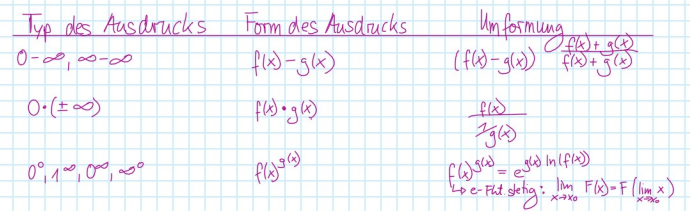
\includegraphics[width=0.8\textwidth]{Bilder/Zusfa/1.png}
\section{Taylor}
Formel:
$$
\begin{matrix}
f(x)=\underbrace{f(x_0)+\frac{f'(x_0)}{1!}\left(x-x_0\right)+\frac{f''(x_0)}{2!}\left(x-x_0\right)^2...+\frac{f^{(n)}(x_0)}{n!}\left(x-x_0\right)^n}_{\text{Taylorpolynom n-ter Ordnung (Hauptteil)}}\\
\\
+\underbrace{\frac{f^{(n+1)}(\xi)}{\left(n+1\right)!}\left(x-x_0\right)^{n+1}}_{R_n \text{Restglied von Lagrange}}
\end{matrix}
$$

Entwicklungspunkt $x_0$ = beliebig, aber fest aus Intervall\\
Zwischenstelle $\xi$ liegt zwischen x und $x_0$, kann also kleiner als x oder auch größer sein.\\
\subsubsection{Fehlerabschätzung}
worst case: $\xi$ zwischen $x_0$ und $x$ so wählen, dass $|R_n(x)|$ größtmöglich wird.\\
$$
\begin{matrix}
\Rightarrow\left|f(x)-P_n(x)\right|=\left|R_n(x)\right| &=& \left|\frac{1}{\left(n+1\right)!}f^{(n+1)}(\xi)\left(x-x_0\right)^{n+1}\right| \\
\\
&=& \frac{1}{\left(n+1\right)!}\left|\left(x-x_09\right)^{n+1}\right|\left|f^{(n+1)}(\xi)\right| \\
\\
&\leq& \frac{1}{\left(n+1\right)!}\left|\left(x-x_09\right)^{n+1}\right| M \\
\end{matrix}
$$
\newpage
Man sieht:\\
1. Je größer das n, dest kleiner wird der Faktor $1\frac{1}{(1-n)!}$\\
auf Deutsch: mit Großerem n wird die approximation besser\\
2. Je weiter das x von $x_0$ weg liegt, desto größer wird der Bertrag $x-x_0$, \\
desto mehr Einfluss hat der Term auf die Genauigkeit\\
\section{Reihen}
\textbf{Die Summe der Glieder einer Folge (oder eines Teils der Folgenglieder) wird als Reihe bezeichnet.}\\
\\
Die Folge $s_n$ nennt man die zur Folge $a_k$ gehörige unendliche
Reihe. Das n-te Glied heißt n-te Partialsumme.
$s_n=\sum\limits_{k=1}^{n}a_k$
Falls die Folge $s_n$ der Partialsummen keinen Grenzwert
besitzt, nennt man die Reihe \textbf{divergent}.
Die Reihe heißt \textbf{konvergent}, wenn $s_n$ konvergiert. 
\\Dann setzt man
$s=\lim\limits_{n\rightarrow \infty}s_n=\lim\limits_{n\rightarrow \infty}\sum\limits_{k=1}^{n}a_k=\sum\limits_{k=1}^{\infty}a_k$
\\Im Falle der Konvergenz sagt man die Reihe $\sum\limits_{k=1}^{\infty}a_k$ ist \textbf{konvergent} und nennt $s$ den Grenzwert die Simme der unendlichen Reihe. 
\subsection{Geometrische Reihe}
$\sum\limits_{k=0}^{\infty}q^k=\frac{1}{1-q},|q|<1$
\\
Für \textcolor{red}{$|q|>1$} wächst der Term $q_n+1$ für $n\rightarrow\infty$ betragsmäßig unbeschränkt,\\ so dass \textbf{Divergenz} der Folge $s_n$ und somit der Reihe vorliegt.
\\
\\
Im Fall \textcolor{red}{$q=1$} gilt für die Partialsumme $s_n=n+1$.\\Damit liegt \textbf{Divergenz} der Reihe vor.
\\
\\
Im Fall \textcolor{red}{$|q|<1$} strebt $q_n+1$ gegen den Grenzwert 0 und die Reihe ist \textbf{konvergent}.
\\
\\
Im Fall \textcolor{red}{$q=-1$} wechselt $s_n$ fortlaufend zwischen den Werten 1 und 0, d.h. es liegt \textbf{Divergenz} vor
\\
\\
\subsection{harmonische Reihe}
$a_k=\frac{1}{\phantom{...}\underbrace{k}_{>0}\phantom{...}}\Rightarrow s_n=a_1+a_2+...+a_n=\overbrace{1+\frac{1}{2}+...+\frac{1}{n}}^{harmonische Reihe}$\\
Die harmonische Reihe ist \textbf{divergent}.
\\\underline{\textbf{\textcolor{red}{Divergenzkriterium:}}}
Falls die Folge $a_k$ \textbf{nicht} gegen Null konvergiert, ist die
unendliche Reihe\\ 
$\sum\limits_{k=1}^{\infty}a_k$ \textbf{divergent.}
Notwendig für die Konvergenz einer Reihe $\sum\limits_{k=1}^{\infty}a_k$ ist die Bedingung, dass die Folge $a_k$
eine \underline{Nullfolge} ist, also $\lim\limits_{k\rightarrow\infty}a_k=0$
\section{Absolute und bedingte Konvergenz von Reihen, Konvergenzkriterien}
Summen und Vielfache konvergenter Reihen ergeben wieder eine konvergente Reihe.
\subsection{bedingte/ absolute Konvergenz}
Die Reihe $\sum\limits_{k=1}^{\infty}a_k$ heißt \textbf{absolut konvergent}, wenn die Reihe der Beträge konvergent ist $\sum\limits_{k=1}^{\infty}|a_k|$
\\
Eine konvergente Reihe, welche nicht absolut konvergent ist, heißt \textbf{bedingt konvergent}.
\\Eine \textbf{absolut konvergente} Reihe ist auch \textbf{(bedingt) konvergent}, die Umkehrung ist i.a. falsch.
\\\underline{\textbf{\textcolor{red}{Majorantenkriterium:}}}\\
$\sum\limits_{k=1}^{\infty}c_k$ konvergente Reihe mit nichtnegativen Gliedern und es gelte $|a_k|\leq c_k$ für alle $k\geq m (fest)$\\
Dann ist die Reihe $\sum\limits_{k=1}^{\infty}a_k$ \textbf{absolut konvergent}.
Bsp:\\
$\sum\limits_{k=1}^{\infty}\frac{k}{k^3+k} \Rightarrow k$ ausklammern $= \frac{k}{k(k^2+1)}=\frac{1}{k^2+1}$
\\Die Reihe verhält sich wie $\sum\limits_{k=1}^{\infty}\frac{1}{k^2}$, sollte daher konvergieren. Begründung:
\\Aus $k^2+1 \geq k^2$ folgt: $\frac{k}{\underbrace{k^3+k}_{=|a_k}}=\frac{1}{k^2+1}\leq \frac{1}{\underbrace{k^2}_{=c_k}}$ 
\\Da nun die Reihe $\sum\limits_{k=1}^{\infty}c_k=\sum\limits_{k=1}^{\infty}\frac{1}{k^2}$ konvergiert, konvergiert auch die Reihe $\sum\limits_{k=1}^{\infty}a_k=\sum\limits_{k=1}^{\infty}\frac{k}{k^3+k}$
\\\underline{\textbf{\textcolor{red}{Minorantenkriterium:}}}\\
$\sum\limits_{k=1}^{\infty}d_k$ divergente Reihe mit nichtnegativen Gliedern und es gelte $a_k\geq d_k$ für alle $k\geq m (fest)$\\
Dann ist die Reihe $\sum\limits_{k=1}^{\infty}a_k$ \textbf{divergent}.
\\Bsp:\\
$\sum\limits-{k=1}^{\infty}\frac{1}{2k-1}$ wächst ähnlich wie $\sum\limits_{k=1}^{\infty}\frac{1}{2k}$\\
Da nun die harmonische Reihe $\sum\limits_{k=1}^{\infty}\frac{1}{k}$ divergiert, divergiert auch die Reihe $\sum\limits_{k=1}^{\infty}\frac{1}{2k}$ und damit auch $\sum\limits_{k=1}^{\infty}\frac{1}{2k-1}$
\\$2k-1\leq 2k \leftrightarrow \frac{1}{\underbrace{2k-1}_{a_k}}\geq \frac{1}{\underbrace{2k}_{=c_k}}$
\\\underline{\textbf{\textcolor{red}{Quotientenkriterium:}}}\\
Gilt für die \textbf{Folge} $a_k$:$\lim\limits_{k\rightarrow \infty}|\frac{a_{k+1}}{a_k}|<1$, dann ist die \textbf{Reihe}: $\sum\limits_{k=1}^{\infty}a_k\leftrightarrow s_n=\sum\limits_{k=1}^{n}a_k$ \textbf{absolut konvergent.}\\
Gilt $\lim\limits_{k\rightarrow \infty}|\frac{a_{k+1}}{a_k}|>1$ ist die Reihe \textbf{divergent.}\\
Gilt $\lim\limits_{k\rightarrow \infty}|\frac{a_{k+1}}{a_k}|=1$ kann man keine Aussage treffen.\\
\\Bsp:\\
Um den Konvergenztest \textbf{Quotientenkriterium} anwenden zu können,
müssen wir aber noch $a_{n+1}$ bestimmen. Dies geschieht ganz einfach dadurch,
dass wir alle $n$ durch $n+1$ ersetzen:\\
\\
$a_n=\frac{3^n}{n^{100}} \rightarrow a_{n+1}=\frac{3^{n+1}}{(n+1)^{100}}$\\
\\
Diese beiden Werte jetzt in das Quotientenkriterium einsetzen:\\
\\
$\lim\limits_{n\rightarrow\infty}|\frac{a_{n+1}}{a_n}|=\lim\limits_{n\rightarrow\infty}|\frac{\frac{3^{n+1}}{(n+1)^{100}}}{\frac{3^n}{n^{100}}}|$\\
\\
Mit den Mitteln der Bruchrechnung vereinfachen wir den Term (Zur Erinnerung:\\
Man dividiert durch einen Bruch, indem man mit dem Kehrwert multipliziert):\\
\\
$\lim\limits_{n\rightarrow\infty}|\frac{a_{n+1}}{a_n}|=\lim\limits_{n\rightarrow\infty}|\frac{3^{n+1}}{(n+1)^{100}}\cdot\frac{n^{100}}{3^n}|$\\
\\
Jetzt multiplizieren wir die beiden Brüche miteinander, wodurch
nur noch ein Bruchstrich übrig bleibt:\\
\\
$\lim\limits_{n\rightarrow\infty}|\frac{a_{n+1}}{a_n}|=\lim\limits_{n\rightarrow\infty}|\frac{3^{n+1}\cdot n^{100}}{(n+1)^{100}\cdot 3^n}|$\\
\\
Jetzt zerlegen wir $3^{n+1}$ mit Hilfe des Potenzgesetzes: $a^{n+m}=a^n\cdot a^m$
Dadurch können wir den Bruch mit $3^n$ kürzen:\\
\\
$\lim\limits_{n\rightarrow\infty}|\frac{a_{n+1}}{a_n}|=\lim\limits_{n\rightarrow\infty}|\frac{\textcolor{blue}{\not{3^n}\cdot 3}\cdot n^{100}}{(n+1)^{100}\cdot \not{3^n}}|=\lim\limits_{n\rightarrow\infty}|\frac{3\cdot n^{100}}{(n+1)^{100}}|$\\
\\
Jetzt dividieren wir Zähler und Nenner jeweils durch $n^{100}$. Im Zähler können
wir dann kürzen, im Nenner wenden wir ein Potenzgesetz an: $a^n/b^n = (a/b)^n$:\\
\\
$\lim\limits_{n\rightarrow\infty}|\frac{a_{n+1}}{a_n}|=\lim\limits_{n\rightarrow\infty}|\frac{\frac{3\cdot \not{n^{100}}}{\not{\textcolor{blue}{n^{100}}}}}{\frac{(n+1)^{100}}{\textcolor{blue}{n^{100}}}}|=\lim\limits_{n\rightarrow\infty}|\frac{3}{(\frac{n+1}{n})^{100}}|$\\
\\
Den Bruch im Nenner schreiben wir auseinander, und können dann kürzen:
\\
$\lim\limits_{n\rightarrow\infty}|\frac{a_{n+1}}{a_n}|=\lim\limits_{n\rightarrow\infty}|\frac{3}{(\frac{\not{n}}{\not{n}}+\frac{1}{n})^{100}}|=\lim\limits_{n\rightarrow\infty}|\frac{3}{(1+\frac{1}{n})^{100}}|$\\
\\
Nun führen wir den Grenzwertübergang durch, d.h. wir ersetzen $n$ überall durch Unendlich:\\
\\
$\lim\limits_{n\rightarrow\infty}|\frac{a_{n+1}}{a_n}|=\lim\limits_{n\rightarrow\infty}|\frac{3}{(1\frac{1}{\infty})^{100}}|=|\frac{3}{(1+0)^{100}}|=|\frac{3}{1}|=\textcolor{blue}{3}$\\
\\
\underline{Ergebnis:}\\
Das Quotientenkriterium liefert den Wert 3 und daher \textbf{divergiert} die gegebene Reihe.
\newpage
\underline{\textbf{\textcolor{red}{Wurzelkriterium:}}}\\
Gilt für die Folge $a_k:\lim\limits_{k\rightarrow\infty}\sqrt[k]{|a_k|}<1$, dann ist die \textbf{Reihe} $\sum\limits_{k=1}^{\infty}a_k$ \textbf{absolut konvergent.}\\
Für $\lim\limits_{k\rightarrow\infty}\sqrt[k]{|a_k|}>1$ gilt \textbf{divergenz}\\
Für $\lim\limits_{k\rightarrow\infty}\sqrt[k]{|a_k|}=1$ kann man keine Aussage treffen.\\
Bsp:\\
$\sum\limits_{n=1}^{\infty}2^{-n}$\\
\underline{1.Betrag:}\\
$|a_n|=|2^{-n}|=2^{-n}$\\
\underline{2.Wurzel nehmen:}\\
$\sqrt[n]{2^{-n}}=(2^{-n})^\frac{1}{n}=2^{-\frac{\textcolor{red}{n}}{\textcolor{red}{n}}}=2^{-1}=\frac{1}{2}$\\
\underline{3.Grenzwert berechnen:}\\
$\lim\limits_{n\rightarrow\infty}\frac{1}{2}=\frac{1}{2}$\\
\textbf{Dieser Wert ist kleiner als 1 ~ also konvergiert die Reihe.}\\
\underline{\textbf{\textcolor{red}{Leibniz-Kriterium für alternierende Reihen:}}}\\
Ist $a_k\geq 0$ eine monoton fallende Folge mit Folge der Eigenschaft $\lim\limits_{k\rightarrow\infty}a_k=0$, dann ist die \textbf{alternierende Reihe}\\
$\sum\limits_{k=1}^{\infty}(-1)^{k+1}a_k=a_1-a_2+a_3-a_4+...$\\
bzw\\
$\sum\limits_{k=1}^{\infty}(-1)^{k}a_k=-a_1+a_2-a_3+a_4-...$\\
\textbf{konvergent.}\\
Bsp:\\
Die alternierende harmonische Reihe $\sum\limits_{k=1}^{\infty}(-1)^{k+1}\frac{1}{k}=1-\frac{1}{2}+\frac{1}{3}-\frac{1}{4}+..$\\
erfüllt die Bedingungen des Leibniz-Kriteriums, denn\\
$a_k=\frac{1}{k}\geq \frac{1}{k+1}=a_{k+1}$und$\lim\limits_{k\rightarrow\infty}a_k=0$\\
\newpage
\section{Potenzreihen}
Eine (reelle) Potenzreihe mit dem Mittelpunkt $x=0$ ist eine \textbf{Reihe} der Form:\\$\sum\limits_{k=0}^{\infty}a_kx^k=a_0+a_1x+a_2x^2+...+a_nx^n+...$\\
Eine (reelle) Potenzreihe mit dem Mittelpunkt \textcolor{red}{oder} Entwicklungspunkt $x=x_0$ ist eine Reihe der Form:\\$\sum\limits_{k=0}^{\infty}a_k(x-x_0)^k=a_0+a_1(x-x_0)+a_2(x-x_0)^2+...+a_n(x-x_0)^n+...$\\
$a_k$ ist eine gegebene (reelle) Zahlenfolge, der Mittelpunkt $x_0$ ist eine reelle Konstante und $x$ ist eine reelle Variable.\\
Bsp:\\
$a_k=1,x_0=2\rightarrow\sum\limits_{k=0}^{\infty}(x-2)^k,x\in\mathbb{R}$\\
$a_k=\frac{1}{k!},x_0=0\rightarrow\sum\limits_{k=0}^{\infty}\frac{1}{k!}x^k,x\in\mathbb{R}$\\
$a_k=\frac{1}{k},x_0=3\rightarrow\sum\limits_{k=1}^{\infty}\frac{1}{k}(x+1)^k,x\in\mathbb{R}$\\
Bsp2:\\
$a_k=1;k=0,1,2,..;x_0=0\rightarrow\sum\limits_{k=0}^{\infty}x^k=1+x+x^2+...+x^k+...$\\\textbf{= Geometrische Reihe}\\
Sie konvergiert für $|x|<1$ gegen $\frac{1}{1-x}$\\
Diese Konvergenz kann man wie folgt ausdrücken:$\sum\limits_{k=0}^{\infty}x^k=\frac{1}{1-x},-1<x<1$\\
Für $|x|\geq 1$ ist die geometrische Reihe \textbf{divergent.}
\subsection{Konvergenzradius}
Jede Potenzreihe $\sum\limits_{k=0}^{\infty}a_k(x-x_0)^k$ besitzt einen eindeutig bestimmten 
\\\textbf{Konvergenzradius} $0\leq p\leq \infty$ mit der Eigenschaft:\\
Die Potenzreihe ist für alle reellen Zahlen $x$ mit:\\
$|x-x_0|<p$ \textbf{absolut konvergent}\\
$|x-x_0|>p$ \textbf{divergent}\\
$|x-x_0|=p$ \textbf{keine Aussage}\\
\textcolor{blue}{$|x-x_0|<p$}$\leftrightarrow$\textcolor{red}{$ -p<x-x_0<p$}$\leftrightarrow$\textcolor{orange}{$ -p+x_0<x<p+x_0$}\\
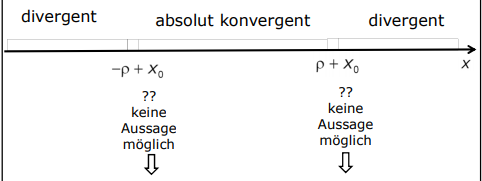
\includegraphics[width=0.8\textwidth]{Bilder/Zusfa/2.png}\\
Konvergenzuntersuchung für die \textbf{Randpunkte} $-p+x_0$ und $p+x_0$ muss separat durchgeführt werden\\
Dazu verwendet man z. B. das Majoranten-/Minorantenkriterium\\
\\
Zur Bestimmung des Konvergenzradius behandelt man Potenzreihen am besten wie gewöhnliche Reihen.\\
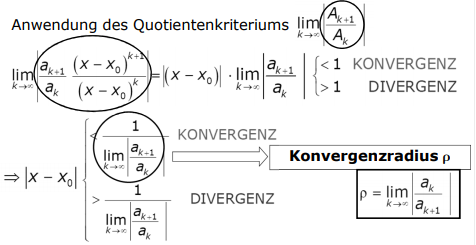
\includegraphics[width=0.8\textwidth]{Bilder/Zusfa/3.png}\\
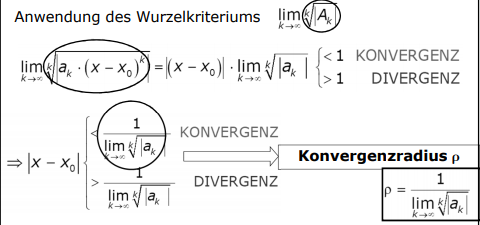
\includegraphics[width=0.8\textwidth]{Bilder/Zusfa/4.png}\\
\textbf{Egal, ob der Konvergenzradius mit dem Quotienten- oder mit
dem Wurzelkriterium bestimmt wird, beide Kriterien liefern
den gleichen Wert.}\\
\\
\\Bsp:\\
$\sum\limits_{k=1}^{\infty}\frac{x^k}{k}$ mit \textcolor{red}{$a_k=\frac{1}{k}$},$x_0=0$,\textcolor{blue}{$a_{k+1}=\frac{1}{k+1}$}\\
$p=\lim\limits_{k\rightarrow\infty}|\frac{\textcolor{red}{a_k}}{\textcolor{blue}{a_{k+1}}}|=\lim\limits_{k\rightarrow\infty}|\frac{1}{k}\frac{k+1}{1}|=\lim\limits_{k\rightarrow\infty}|1+\frac{1}{k}|=1$\\
Die Potenzreihe ist für alle reellen Zahlen $x$ mit $|x|<p=1$ \textbf{absolut konvergent}\\
Für $x=1$ gilt: harmonische Reihe $\rightarrow$ \textbf{divergent}\\
Für $x=-1$ gilt: alternierende harmonische Reihe $\rightarrow$ \textbf{konvergent nach Leibniz}
\subsection{Stetigkeitssatz}
Hat die Potenzreihe $\sum\limits_{k=0}^{\infty}a_k(x-x_0)^k$ den \textbf{Konvergenzradius} $p$, so ist die Potenzreihe für $|x-x_0|<p$ stetig.
\\
\\
\underline{Satz3:}\\
Besitzen die beiden Potenzreihen $\sum\limits_{k=0}^{\infty}a_kx^k,\sum\limits_{k=0}^{\infty}b_kx^k$ die Konvergenzradien $p_a$ bzw. $p_b$, dann dürfen die Potenzreihen im Inneren des kleineren Konvergenzintervalls\\
$p=min\{p_a,p_b\} $ \\
gliedweise addiert bzw. subtrahiert und gliedweise mit einer Zahl $\alpha$ multipliziert werden.\\
Die daraus entstehenden Potenzreihen:\\
$\sum\limits_{k=0}^{\infty}a_kx^k+\sum\limits_{k=0}^{\infty}b_kx^k=\sum\limits_{k=0}^{\infty}(a_k+b_k)x^k,\alpha\sum\limits_{k=0}^{\infty}a_kx^k=\sum\limits_{k=0}^{\infty}\alpha a_kx^k$\\
haben ebenfalls den Konvergenzradius $p>0$
\\
Das gilt auch für die \textbf{Ableitung}

\end{document} 